\documentclass[10pt]{article}
\usepackage[utf8]{inputenc}
\usepackage[shortlabels]{enumitem}
\usepackage[margin=1in]{geometry}
\usepackage{setspace}
\usepackage{hyperref}
\usepackage{graphicx}
\onehalfspacing
\setlength{\parskip}{1em}
\setlength{\parindent}{0pt}
\bibliographystyle{ecta}
\usepackage[T1]{fontenc}
\usepackage{titling}
\usepackage{amsmath}
\setlength{\droptitle}{-7em}
\addtolength\abovedisplayskip{-3in}
\addtolength\belowdisplayskip{-3in}

\title{City Location Choice and Household Productivity}
\preauthor{}
\postauthor{}
\author{Tan Sein Jone}
\predate{}
\postdate{}
\date{}
%\Today

\begin{document}
\doublespacing
\maketitle

% \section{Model}

% \subsection{Joint distribution of productivity across cities}

% \begin{align}
%     P[Z_c \leq z]                    & = e^{-G^c T_c z^{-\theta}}                                                            \\
%     P[Z_1 \leq z, \dots, Z_c \leq z] & = exp[-\sum_{c = 1}^{N}(G^c Z_c T_{c}^{-\theta})^{\frac{1}{1 - \sigma}}]^{1 - \sigma}
% \end{align}

% $G^c$ is the tail dependence correlation funciton. $\sigma$ determines the substitutability between cities.$Z_c$ is the exogenous productivity of households. $\theta$ is the shapre parameter.

% \subsection{Tail dependence correlation function}

% \begin{align}
%     G^c(x_1, \dots, x_c) = \sum_{k = 1}^{K}[\sum_{s = 1}^{N}(w_{sk}x_{sc})^{\frac{1}{1 - \rho_k}}]^{1 - \rho_k}
% \end{align}

% $w_{sk}$ is the weight of technology $k$ for sector $s$ which is common between cities. $\rho_k$ is the substitutability of technologies. $x_{s}^{c}$ is the expenditure in sector $s$ for city $c$, this can be analogous to endowments for each city.

% \subsection{Individual distributions}

% \begin{align}
%     P[T_{csk} \leq t] = exp [-((w_{sk} x_{sc})^{\frac{1}{1 - \rho_k}} Z_c T_{c}^{-\theta})^{\frac{1}{1 - \sigma}}]
% \end{align}

% Specific Fréchet distribution for city $c$, sector $s$ and technology $k$.

% \begin{equation}
%     \phi_c =
%     \begin{pmatrix}
%         t_{11} & \cdots & t_{1k} \\
%         \vdots & \ddots & \vdots \\
%         t_{s1} & \cdots & t_{sk}
%     \end{pmatrix}
% \end{equation}

% $\phi_c$ is the matrix of productivity draws from their respective Frechet distributions for each sector and technology in city $c$.

% \subsection{Individual specific technology endowments}

% \begin{equation}
%     \omega_p =
%     \begin{pmatrix}
%         v_{1}  & \\
%         \vdots & \\
%         v_{k}  &
%     \end{pmatrix}
% \end{equation}

% $\omega_p$ is the vector of technology endowments for each person $p$. For now, each endowment is assumed to be drawn from a normal distribution.

% \newpage

% \section{Aggregation Consideration}

% \subsection{Expected City Wage Realization}

% \begin{align}
%     E[w_c | \omega_p, \phi_c] = A_c[\sum_{s}^{}(T_s \sum_{k}^{} v_{sk} z_{sk})^{\frac{\eta}{\eta - 1}}]^{\frac{\eta - 1}{\eta}}
% \end{align}

% Realised wage for person $p$ in city $c$ given their technology draws and the productivity draws for the city.

% $T_s$ will be a sector specific scale parameter that is analogous to a city's amenities which is determined by a person's preference towards a specific sector. $A_c$ is a city specific amenity shifter.

% \subsection{Worker problem}

% \begin{align}
%     \max_{w} [E[w_1 | \omega_p, \phi_1], \dots, E[w_N | \omega_p, \phi_N]]
% \end{align}

% The worker will choose the city that maximizes their expected wage.

% \newpage

\section{Introduction}

The location choice of households across cities is a fundamental question in urban economics. The choice of location is dependent on a variety of factors such as amenities, housing costs, and job opportunities. Quantitative spacial models such as the one developed by Redding (2016) have been able to explain the distibution of economic activity acorss cities by intergrating an amenity shifter into their model. We believe however that the distribution of economic activity across cities is also dependent on the distribution of job types across cities. With cities specializing in specific occupations attracting houeholds that are most productive in those occupations. This means that only cities that are most simillar in their technologies, relfected in their employment structure, will be able to attract hosueholds of specific types. In order to break the independence of irrelevant alternatives (IIA) assumption, we look to Lind and Ramondo (2023) who have developed an EK model with multiple technologies to produce correlated productivity draws across countries.

\subsection{Literature Review}

Eaton and Kortum (2022) present a quantitative trade model that incorporates Ricardian motives for trade by treating productivity as random draws acorss goods, countries and other observable units. This model however relies on indepndence asusmptions that don't capture the relavent substiution patterns for goods acorss countries. Specifically, the dynamic where countries with the most simillar technologies trade most with each other.

Lind and Ramondo (2023) overcome this limitation by developing an EK model with multiple technologies that produce correlated productivity draws across countries. This is achieved using a corss nested constant-elasticity-of-substitution (CES) structure for productivity, with latent nests having the interpretation of technologies. Sectors in countries can then share technologies, which allows for the correlation of productivity draws across countries.

\section{Model of Production}

\begin{align}
    Y_{ck} (\nu) = Z_{ck}(\nu)
\end{align}

Consider a closed economy consisting of $N$ cities and a continnium of household types $\nu \in [0, 1]$ . Each city $c$ employs hosueholds of type $\nu$ in occupation $k$ to produce output $Y_{ck}(\nu)$. We assume no trade costs between cities, and that the price of the good produced by occupation $k$ is freely traded and priced under perfect competition. The price index of city $c$ is $\Phi_c$. The wage of a worker in sector $k$ in city $c$ is $w_{ck}(\nu) = \Phi_c Z_{ck}(\nu)$. As in EK, productivity is a random variable drawn from a max stable multivariate Fréchet distribution and is dependent on both the city and occupation. Output by a specifc occupation is assumed to be produced by a random sector.

% \begin{align}
%     Y_{s | c} = T_{cs} \prod_{k} Q_{sk}^{\omega_{sk}}
% \end{align}

% The economy consists of $s \in S$ sectors which employ occupations/tasks according to a Cobb-Douglas production function. $\omega_{sk}$ is the weight that each occupation takes for every sector, where $\sum_{k}^{} \omega_{sk} = 1$ for each sector $s$. $T_{cs}$ is some exogenous productivity associated with a city-sector pair (Detriot and automanufacturing, for example).

% \subsection{MRP}

% \begin{align}
%     {MRP}_{csk}(\nu) = {p_{s}}{T_{cs}}{\omega_{sk}}{z_{k}(\nu)}
% \end{align}

% The world consists of some continuum of householdslds $\nu \in [0, 1]$. Households exhibit some productivity for a range of occupations/tasks, denoted $k \in K$. For worker $\nu$, their productivity in $k$ is $z_{k}(\nu)$. Each worker therefore faces a marginal revenue product associated with being employed in occupation $k$ within sector $s$ in city $c$.

% $p_{s}$ is the price of the good produced by sector $s$, which we assume is freely traded and priced under perfect competition. That is, the price of $s$ is identical in all cities. We assume that when households choose a city $c$ they are randomly assigned to a sector $s$ depending on the employment shares within that city accruing to sector $s$: $\phi_{cs}$. Notice that $\phi_{cs}$ is related to $T_{cs}$, and for now we make the simplifying assumption that:

% \begin{align}
%     \phi_{cs} = \frac{T_{cs}}{\sum_{s}^{} T_{cs}}
% \end{align}

% The marginal revenue product of being employed in occupation $k$ in city $c$ for household $\nu$ is therefore the following:

% \begin{align}
%     {MRP}_{ck}(\nu) = {z_{k}(\nu)}\sum_{s}^{} p_{cs} \phi_{cs} T_{cs} \omega_{sk}
% \end{align}

% Finally, we separate $T_{cs}$ into a city-specific component which applies to all sectors, $T_{c}$, and an idiosyncratic component that is city-sector specific, $\tilde{T}_{cs}$. We can therefore re-write our expected marginal revenue product of worker $\nu$ working in occupation $k$ in city $c$ as:

% \begin{align}
%     {MRP}_{ck}(\nu) = {z_{k}(\nu)}{T_{c}}{B_{ck}}
% \end{align}

% where $B_{ck} = \sum_{s}^{} p_{s} \phi_{cs} \tilde{T}_{cs} \omega_{sk}$ and captures the employment structure in city $c$ and how attractive this structure is to a worker in occupation $k$.

% From here, we will aggregate over all occupations in a city to derive the expected wage for a worker in city $c$.

% \begin{align}
%     MRP_c(\nu) = \sum_{k}^{} [z_{k}(\nu)T_{c}B_{ck}]
% \end{align}

\section{Max Stable Multivariate Fréchet Distribution}

We assume that the joint distribution of productivity across cities is given by

\begin{align}
    P[Z_{1k}(\nu) < z, \dots, Z_{Nk} (\nu) < z] = exp[-\sum_{c}^{N}(T_{ck} H_k(\nu) z^{-\theta})^{\frac{1}{1 - \rho_k}}]^{1 - \rho_k}
\end{align}

Where $T{ck}$ is the scale parameter for city $c$ and occupation $k$, this represents a city's absolute advantage for occupation $k$. $H_k(\nu)$ is the occupation specific productivity shifter for household of type $\nu$ in occupation $k$, the heterogeneity of this shifter relfects the difference in human capital across different hosuehold types. $\theta > 0$ is the shape parameter, characaterizing the tail behavior of the distribution. $\rho_k$ is the occupation specific correlation parameter, which dictates the extent to which productivity draws are correlated across cities for occupation $k$.

A household's schedule of productivities is characterized by a vector of draws from different Fréchet distributions for each city occupation pair. The realized productivity a hosuehold of type $\nu$ has in city $c$ is the occupation that maximizes the producticity that particular household has in the city. This is given by the following:

\begin{align}
    Z_c(\nu) = \max_{k} \{Z_{ck}(\nu)\}
\end{align}

Unlike sequential games where households might pick a city before picking an occupation, this schedule of productivity already determines the ideal occupation for a household in a city. The joint probability of all productivities being less than some value $z$ for all cities is then given by the following:

\begin{align}
    P[Z_1(\nu) < z, \dots, Z_N(\nu) < z] = exp\{- \sum_{k}^{}[\sum_{c}^{N}(T_{ck} H_k(\nu) z^{-\theta})^{\frac{1}{1 - \rho_k}}]^{1 - \rho_k}\}
\end{align}

The joint probability above is a max-stable multivariate Fréchet distribution with a cross-nested CES correlation function. This distribution is a generalization of the Fréchet distribution to the multivariate case, and is used to model the joint distribution of extreme values. This is simillar to the GEV distribution, but with the added feature of a correlation function that allows for the dependence of extreme values across occupations. A houehold of type $\nu$ has realised productivity that is hence characterised by the maxmimum productivity draw across all cities scaled by the inverse of that city's price index $\Phi_c$ and is gievn by the following:

\begin{align}
    Z(\nu) = \max_{c = 1, \dots, N} \left\{\frac{Z_c(\nu)}{\Phi_c}\right\}
\end{align}

\subsection{Correlation Function}

\begin{align}
    P[Z_{1k} < z, \dots, Z_{Nk} < z] = exp[-\sum_{c}^{N}(T_{ck} z^{-\theta})^{\frac{1}{1 - \rho_k}}]^{1 - \rho_k}
\end{align}

\begin{align}
    P[Z_1 < z, \dots, Z_N < z] = exp\{- \sum_{k}^{}[\sum_{c}^{N}(T_{ck} z^{-\theta})^{\frac{1}{1 - \rho_k}}]^{1 - \rho_k}\}
\end{align}

When we intergrate over all houehold types for a particular occupation shifter, we get some average productivity shifter for that occupation. $\int_{0}^{1} H_k (\nu) d\nu = 1$. With the case of a cross-nested CES function, we can approximate a correlation funciton. Assuming that productivity is distributed max-stable multivariate Fréchet, with scale parameter $T_{ck}$, shape parameter $\theta$, and correlation parameter $\rho_k$, we can assume the following correlation function:

\begin{align}
    G (Z_1^{-\theta}, \dots, Z_N^{-\theta})= \sum_{k}^{} [\sum_{c}^{N} (T_{ck} Z_c^{-\theta})^{\frac{1}{1 - \rho_k}}]^{1 - \rho_k}
\end{align}

\begin{align}
    G_c (Z_1^{-\theta}, \dots, Z_N^{-\theta}) = \frac{\partial G (Z_1^{-\theta}, \dots, Z_N^{-\theta})}{\partial Z_c^{-\theta}}
\end{align}

\begin{align}
    \gamma = \Gamma (\frac{\theta - 1}{\theta})
\end{align}

Where $G_c$ is the derivative of the correlation function with respect to city $c$. This correlation function is a generalization of the CES correlation function to the multivariate case, and is used to model the dependence of extreme values across cities. The $\Gamma$ function which takes in the ratio of $\theta - 1$ to $\theta$ gives us the substitutability between cities. Productivity is related to $\gamma$ by the following funciton:

\begin{align}
    Z_c^{-\theta} = (\gamma \Phi_c)^{-\theta} T_c
\end{align}

Where $T_c$ is the city's absolute advantage that applies to all occupations and is given by $T_c = \sum_{k}^{} T_{ck} H_k$.

\subsection{Choice Shares}

Under perfect competition, wages are equal to marginal revenue product and is a direct function of productivity. As established in equation (5), the productivity for a worker $\nu$ in city $c$ is given by the maximum productivity draw across all occupations. All we have to do is intergrate over all houshold types to get the productivity index for city $c$:

\begin{align}
    Z_c = \max_k \left\{ \int_{0}^{1} Z_{ck} (\nu) d\nu \right\}
\end{align}

If productivity is distributed max-stable multivariate Fréchet and a continiously differentiable correlation function, then city $c$'s choice shares for a given occupaiton $k$ is given by the following:

\begin{align}
    \pi_{ck} = \frac{Z_c^{-\theta} G_c^k(Z_1^{-\theta}, \dots, Z_N^{-\theta})}{G^k(Z_1^{-\theta}, \dots, Z_N^{-\theta})}
\end{align}

Where $G^k (Z_1^{-\theta}, \dots, Z_N^{-\theta}) = [\sum_{c}^{N} (T_{ck} Z_c^{-\theta})^{\frac{1}{1 - \rho_k}}]^{1 - \rho_k}$

The share of location choices for households has the same form as choice probabilities in GEV discrete choice models, with $Z_c^{-\theta}$ replacing choice specific utility. As in EK, the share of location choices of city $c$ equals the probability that a worker is most productive in city $c$. Finally, the location choice share in each city is determined by the ratio of the expected productivity in that city to the expected productivity in all cities.

\begin{align}
    \pi_{ck} = \frac{(T_{ck} Z_c^{-\theta})^{\frac{1}{1 - \rho_k}}}{\sum_{c}^{N} (T_{ck} Z_c^{-\theta})^{\frac{1}{1 - \rho_k}}}
\end{align}

% When aggregating over all occupations, the share of location choices for city $c$ is given by the following:

% \begin{align}
%     \pi_c = \frac{\sum_{k}^{} (\pi_{ck})^{1 - \rho_k}}{\sum_{k}^{} \sum_{c}^{N} (\pi_{ck})^{1 - \rho_k}}
% \end{align}

Now for a city's aggreagte choice shares. We make the simplifying asusmption that $\rho_k = \rho$ for all occupaitons $k$. This allows us to begin with the following expressions:

\begin{align}
    G(Z_1^{-\theta}, \dots, Z_N^{-\theta})   & = \sum_{k}^{}[\sum_{c}^{N}(T_{ck} Z_c^{-\theta})^{\frac{1}{1 - \rho}}]^{1 - \rho}                       \\
    G_c(Z_1^{-\theta}, \dots, Z_N^{-\theta}) & = \frac{\partial G(Z_1^{-\theta}, \dots, Z_N^{-\theta})}{\partial Z_c^{-\theta}}                        \\
    \pi_c                                    & = \frac{Z_c^{-\theta} G_c(Z_1^{-\theta}, \dots, Z_N^{-\theta})}{G(Z_1^{-\theta}, \dots, Z_N^{-\theta})}
\end{align}

% We then evaluate equation (16) to get:

% \begin{align}
%     \frac{\partial G(Z_1^{-\theta}, \dots, Z_N^{-\theta})}{\partial Z_c^{- \theta}} = \sum_{k}^{} \left[ \lambda_k^{- \rho} (T_{ck} Z_c^{- \theta})^{\frac{1}{1 - \rho}} (Z_c^{- \theta})^{- 1} \right]
% \end{align}

% Where $\lambda_k = \sum_{c}^{N} (T_{ck} Z_c^{-\theta})^{\frac{1}{1 - \rho_k}}$.

% Plugging in the expression for $G_c$ into equation (17), we get the following:

Evaluating expression (17), we get the following:

\begin{align}
    \pi_c = (Z_c^{- \theta})^{\frac{1}{1 - \rho}} \left[ \frac{\sum_{k}^{} T_{ck}^{\frac{1}{1 - \rho}} \lambda_k^{- \rho}}{\sum_{k}^{} \lambda_k^{1 - \rho}} \right]
\end{align}

\subsection{Substitutability}

In the case of a cross nested CES function, we can approximate the substitutability between cities within a given occupation. We can do this by taking the log derivative of the choice share of city $c$ with respect to the city's absolute advantage $T_{ck}$. Solving for the derivative of Equation (14) with respect to $ln (T_{ck})$, we get the following:

\begin{align}
    \frac{\partial ln \pi_{ck}}{\partial ln T_{c'k}} = - \frac{1}{1 - \rho_k} \frac{1}{T_{c'k}} \pi_{c'k}
\end{align}

We can see that for any given occupation, the substitutability between cities is determined by the correlation parameter $\rho_k$, the city's absolute advantage $T_{c'k}$, and the choice share of that city $\pi_{c'k}$. As occupations are more correlated, cities become more substitutable. As any given city's share increases, the substitutability increases. This illustrates a gravity effect where cities that are more productive in a given occupation and hence have a larger share of houeholds are more likely to further attract more households for that occupation.

When we evaluate the own price "own price" elasticity of city $c$'s choice share with respect to the city's absolute advantage $T_{ck}$, we make the simplifying assumption that each city is small and therefore $\frac{\partial \lambda_k}{\partial T_{ck}} = 0$. This gives us the following expression:

\begin{align}
    \frac{\partial ln \pi_{ck}}{\partial ln T_{ck}} \approx \left( \frac{1}{1 - \rho} \right) \left[ \frac{\partial ln Z_c^{- \theta}}{\partial ln T_{ck}} +\frac{T_{ck}^{\frac{1}{1 - \rho}} \lambda_k^{- \rho}}{\sum_{k}^{} T_{ck}^{\frac{1}{1 - \rho}} \lambda_k^{-\rho}} \right]
\end{align}

Simmilarly, we can get the cross price elasticity of city $c$'s choice share with respect to that city's absolute advantage $T_{c'k}$:

\begin{align}
    \frac{\partial ln \pi_c}{\partial ln T_{c'k}} \approx - \pi_{c'k} \left[ 1 + \left( \frac{\rho}{1 - \rho} T_{ck}^{\frac{1}{1 - \rho}} \right) \right]
\end{align}

\section{Simulations}

Assume now that we have two occupations trades and services. We will also assume three cities, Detriot, Chicago and New York with Detriot and Chicago specializing in trades and New York specializing in services. We will also assume that the correlation parameter $\rho_k$ is 0.7 for trades and 0.5 for services and the shape parameter $\theta$ is 2. This will give us the folliwing scale parameters for cities and hosuehold types:

\vspace{2em}

% \begin{table}[h]
%     \begin{minipage}{0.5\textwidth}
%         \centering
%         \begin{tabular}{|l|c|c|c|}
%             \hline
%                               & \textbf{Detriot} & \textbf{Chicago} & \textbf{New York} \\
%             \hline
%             \textbf{Trades}   & 7                & 8                & 3                 \\
%             \hline
%             \textbf{Services} & 2                & 1                & 8                 \\
%             \hline
%         \end{tabular}
%         \caption{City Scale Parameters $T_{ck}$}
%         \label{city_shifter}
%     \end{minipage}%
%     \begin{minipage}{0.5\textwidth}
%         \centering
%         \begin{tabular}{|l|c|c|c|}
%             \hline
%                               & \textbf{$\nu_1$} & \textbf{$\nu_2$} \\
%             \hline
%             \textbf{Trades}   & 7                & 4                \\
%             \hline
%             \textbf{Services} & 3                & 8                \\
%             \hline
%         \end{tabular}
%         \caption{Houshold Scale Parameter $H_k(\nu)$}
%         \label{household_shifter}
%     \end{minipage}
% \end{table}

\begin{table}[h]
    \centering
    \begin{tabular}{|l|c|c|c|}
        \hline
                          & \textbf{Detriot} & \textbf{Chicago} & \textbf{New York} \\
        \hline
        \textbf{Trades}   & 7                & 8                & 3                 \\
        \hline
        \textbf{Services} & 2                & 1                & 8                 \\
        \hline
    \end{tabular}
    \caption{City Scale Parameters $T_{ck}$}
    \label{city_shifter}
\end{table}

\vspace{2em}

These shifters will determine the Frechet distributions from which city and occupation specific productivities are drawn for each household type. For context, this is the pdf for each of the Frechet distributions:

\begin{align}
    P[Z_{ck} < z] = exp[-(T_{ck} z^{-\theta})^{\frac{1}{1 - \rho_k}}]
\end{align}

For each household, the draws will produce a $K \times N$ matrix which reflects that hosuehold's schedule of productivities across all cities and occupations. The realized productivity for each household is then the maximum productivity draw across all cities and occupations. Location choice is hence the column which contains that realised productivity.

% \begin{figure}[h]
%     \begin{minipage}{0.5\textwidth}
%         \centering
%         \includegraphics[width=\textwidth]{../simulations/graphs/city_pop.png}
%         \caption{Initial Distribution of Populations}
%         \label{city_pop}
%     \end{minipage}%
%     \begin{minipage}{0.5\textwidth}
%         \centering
%         \includegraphics[width=\textwidth]{../simulations/graphs/c_shock.png}
%         \caption{Post Detriot Shock}
%         \label{c_shock}
%     \end{minipage}
% \end{figure}

% \begin{figure}
%     \centering
%     \includegraphics[width=\textwidth]{../../simulations/graphs/city_pop.png}
%     \caption{Initial Distribution of Populations}
%     \label{city_pop}
% \end{figure}

% \begin{figure}
%     \centering
%     \includegraphics[width=\textwidth]{../../simulations/graphs/c_shock.png}
%     \caption{Post Detroit Shock}
%     \label{c_shock}
% \end{figure}

We now draw 10000 households, simulating the dtstribution of location choices across cities. As shown in figure 1, the city with the highest population is New York, with the majority of service focused households choosing to locate in the city. Detriot and Chicago have a more even distribution of trades focused households.

We then shock Detriot's productivities, reducing it by $50\%$ and observe the change in location choices. As shown in figure 2, there is a redistibution in location choices with the majority of trades focused households now choosing to locate in Chicago. Some households have also chosen to locate in New York due to higher productivity draws in that city.

\subsection{Numerical vs Analytical Results Comparison}

Given the generation of synthetic reuslts, this gives us the opportunity to compare the numerical results with the analytical results. We can compare the choice shares of each city as given by the analytical model with the choice shares of each city as given by the numerical model. This will allow us to validate the analytical model and see if it is able to capture the distribution of location choices across cities.

% \begin{figure}
%     \begin{minipage}{0.5\textwidth}
%         \centering
%         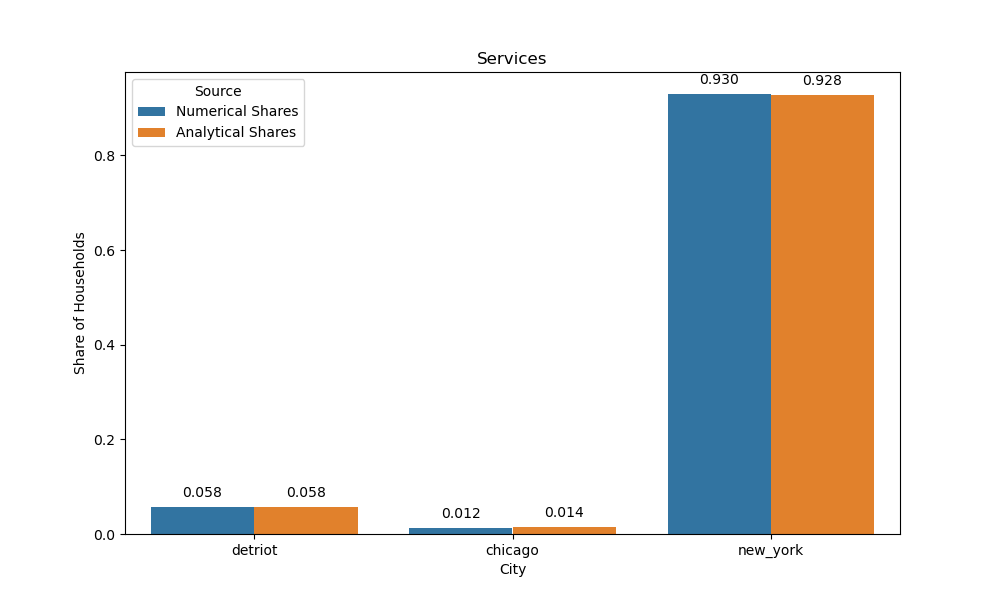
\includegraphics[width=\textwidth]{../../simulations/graphs/sim_services.png}
%         \caption{Service Choice Shares}
%         \label{sim_services}
%     \end{minipage}
%     \begin{minipage}{0.5\textwidth}
%         \centering
%         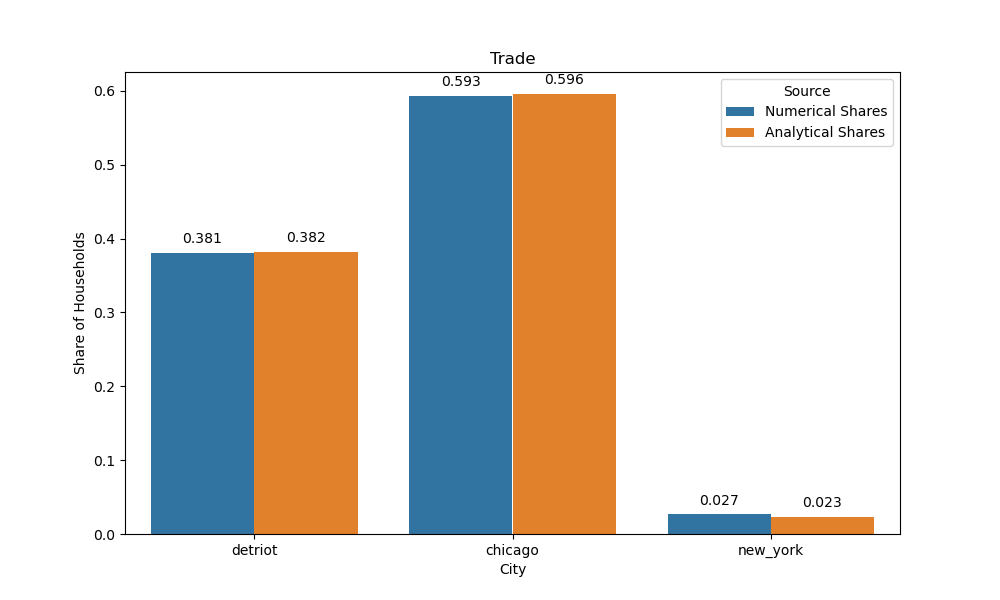
\includegraphics[width=\textwidth]{../../simulations/graphs/sim_trade.png}
%         \caption{Trades Choice Shares}
%         \label{sim_trades}
%     \end{minipage}
% \end{figure}

As you can see in figures 3 and 4, the analytical model is able to capture the distribution of location choices across cities. The choice shares of each city as given by the analytical model are very simillar to the choice shares of each city as given by the numerical model. This validates the analytical model and shows that it is able to capture the distribution of location choices across cities.

The same excercise can be done for the choice shares for each city. We compare the choice shares for each city as given by the analytical model with the choice shares for each city as given by the numerical model in order to validate the analytical model.

% \begin{figure}
%     \centering
%     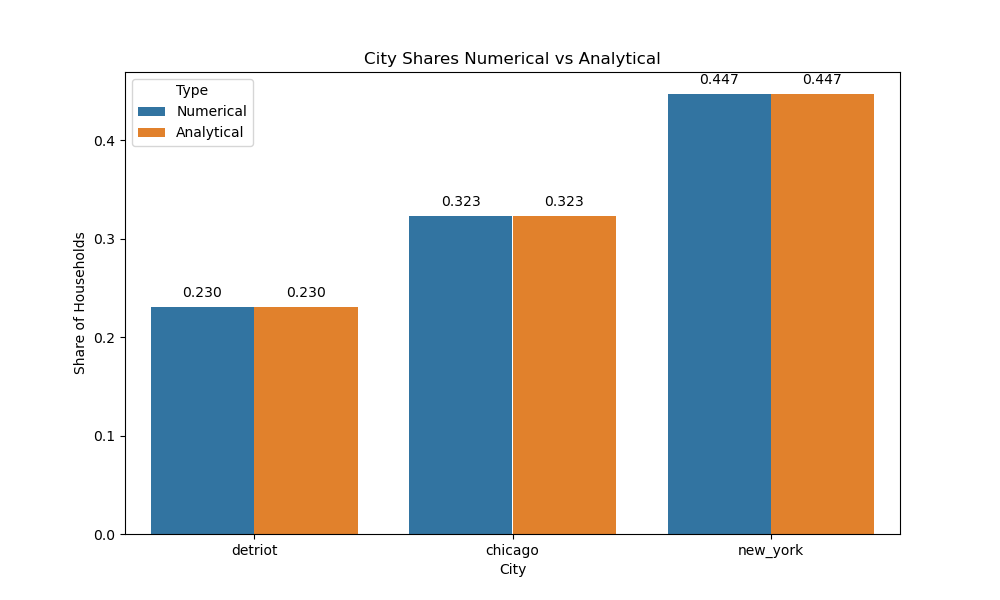
\includegraphics[width=\textwidth]{../../simulations/graphs/sim_city_shares.png}
%     \caption{City Choice Shares}
%     \label{sim_city_shares}
% \end{figure}

As shown in figure 5, the analytical model is able to capture the distribution of location choices across cities. While the shares are not exactly the same, the analytical model is able to capture the general distribution of location choices across cities. This validates the analytical model and shows that it is able to capture the distribution of location choices across cities.

\newpage

\section{Proofs}

\subsection{Proof of Equation (14)}

% \begin{align*}
%     G_c (Z_1^{-\theta}, \dots, Z_N^{-\theta})               & = \frac{\partial G(Z_1^{-\theta}, \dots, Z_N^{-\theta})}{\partial Z_c^{-\theta}}                                 \\
%                                                             & = \sum_{k}^{} [(T_{ck} )^{\frac{1}{1 - \rho_k}} (Z_c^{-\theta})^{\frac{1}{1 - \rho_k} - 1}]^{1 - \rho_k} \\
%                                                             & = Z_c^{-\theta} \sum_{k}^{} [(T_{ck} Z_c^{-\theta} )^{\frac{1}{1 - \rho_k}}]^{1 - \rho_k}                \\
%                                                             & = Z_c^{-\theta} \sum_{k}^{} T_{ck} Z_c^{-\theta}                                                         \\
%     Z_c^{-\theta} G_c (Z_1^{-\theta}, \dots, Z_N^{-\theta}) & = \sum_{k}^{} T_{ck}  Z_c^{-\theta}
% \end{align*}

% \begin{align*}
%     \frac{Z_c^{-\theta} G(Z_1^{-\theta}, \dots, Z_N^{-\theta})}{G(Z_1^{-\theta}, \dots, Z_N^{-\theta})} & = \frac{\sum_{k}^{} T_{ck} Z_c^{-\theta}}{\sum_{k}^{} [\sum_{c}^{N} (T_{ck} Z_c^{-\theta})^{\frac{1}{1 - \rho_k}}]^{1 - \rho_k}}      \\
%                                                                                                         & = \frac{\sum_{k}^{} T_{ck} Z_c^{-\theta}}{\sum_{c}^{N} \sum_{k}^{} (T_{ck} Z_c^{-\theta})^{\frac{1}{1 - \rho_k} \times (1 - \rho_k)}} \\
%                                                                                                         & = \frac{T_c Z_c^{-\theta}}{\sum_{c}^{N} T_c Z_c^{-\theta}}                                                                            \\
%                                                                                                         & = \frac{T_c Z_c^{-\theta}}{\sum_{c}^{N} T_c Z_c^{-\theta}}
% \end{align*}

\begin{align*}
    G^k (Z_1^{-\theta}, \dots, Z_N^{-\theta})                                                                    & =  [\sum_{c}^{N} (T_{ck} Z_c^{-\theta})^{\frac{1}{1 - \rho_k}}]^{1 - \rho_k}                                                                                                                     \\
    G_c^k (Z_1^{-\theta}, \dots, Z_N^{-\theta})                                                                  & = \frac{\partial G(Z_1^{-\theta}, \dots, Z_N^{-\theta})}{\partial Z_c^{-\theta}}                                                                                                                 \\
                                                                                                                 & = (1 - \rho_k)[\sum_{c}^{N} (T_{ck} Z_c^{- \theta})^{\frac{1}{1 - \rho_k}}]^{- \rho_k} (\frac{1}{1 - \rho_k} (T_{ck} Z_c^{- \theta})^{\frac{1}{1 - \rho_k} - 1} T_{ck})                          \\
                                                                                                                 & = (1 - \rho_k) \frac{1}{1 - \rho_k} \frac{T_{ck}}{T_{ck} Z_c^{- \theta}} (T_{ck} Z_c^{- \theta})^{\frac{1}{1 - \rho_k}} [\sum_{c}^{N} (T_{ck} Z_c^{- \theta})^{\frac{1}{1 - \rho_k}}]^{- \rho_k} \\
    Z_c^{- \theta} G_c^k (Z_1^{-\theta}, \dots, Z_N^{-\theta})                                                   & = \frac{(T_{ck} Z_c^{-\theta})^{\frac{1}{1 - \rho_k}}}{\sum_{c}^{N} (T_{ck} Z_c^{-\theta})^{\frac{1}{1 - \rho_k}}} [\sum_{c}^{N} (T_{ck} Z_c^{-\theta})^{\frac{1}{1 - \rho_k}}]^{1 - \rho_k}     \\
    \frac{Z_c^{- \theta} G_c^k (Z_1^{-\theta}, \dots, Z_N^{-\theta})}{G^k (Z_1^{-\theta}, \dots, Z_N^{-\theta})} & = \frac{(T_{ck} Z_c^{-\theta})^{\frac{1}{1 - \rho_k}}}{\sum_{c}^{N} (T_{ck} Z_c^{-\theta})^{\frac{1}{1 - \rho_k}}}                                                                               \\
    \pi_{ck}                                                                                                     & = \frac{(T_{ck} Z_c^{-\theta})^{\frac{1}{1 - \rho_k}}}{\sum_{c}^{N} (T_{ck} Z_c^{-\theta})^{\frac{1}{1 - \rho_k}}}
\end{align*}

\subsection{Substitutability Proof}

\begin{align*}
    \frac{\partial ln \pi_{ck}}{\partial ln T_{ck}} & = \frac{1}{1 - \rho_k} - \frac{\frac{1}{1 - \rho_k} (T_{ck} Z_c^{- \theta})^{\frac{1}{1 - \rho_k} - 1}}{\sum_{c}^{N} (T_{ck} Z_c^{-\theta})^{\frac{1}{1 - \rho_k}}}            \\
                                                    & = \frac{1}{1 - \rho_k} \left[1 - \frac{1}{T_{ck}} \frac{(T_{ck} Z_c^{- \theta})^{\frac{1}{1 - \rho_k}}}{\sum_{c}^{N} (T_{ck} Z_c^{-\theta})^{\frac{1}{1 - \rho_k}}}\right] > 0 \\
\end{align*}

\begin{align*}
    \frac{\partial ln \pi_{ck}}{\partial ln T_{c'k}} & = - \frac{1}{1 - \rho_k} \frac{1}{T_{c'k}} \frac{(T_{c'k} Z_{c'}^{- \theta})^{\frac{1}{1 - \rho_k}}}{\sum_{c}^{N} (T_{ck} Z_c^{-\theta})^{\frac{1}{1 - \rho_k}}} \\
                                                     & = - \frac{1}{1 - \rho_k} \frac{1}{T_{c'k}} \pi_{c'k} < 0
\end{align*}

\subsection{Estimation Equation}

\begin{align*}
    \pi_{ck}    & = \frac{(T_{ck} Z_c^{- \theta})^{\frac{1}{1 - \rho_k}}}{\sum_{c}^{N} (T_{ck} Z_c^{- \theta})^{\frac{1}{1 - \rho_k}}}                         \\
    ln \pi_{ck} & = \frac{1}{1 - \rho_k} \left[ln (T_{ck}) + ln\left\{(\gamma \Phi_c)^{- \theta} \sum_{k}^{} T_{ck}\right\}\right] - ln \left[\Lambda_k\right] \\
\end{align*}

Where $\Lambda_k = \sum_{c}^{N} (T_{ck} Z_c^{- \theta})^{\frac{1}{1 - \rho_k}}$. And $Z_{ck}^{- \theta} = (\gamma \Phi_c)^{- \theta} T_c$.

% \begin{align*}
%     \pi_{ck}                   & = \frac{(T_{ck} Z_c^{-\theta})^{\frac{1}{1 - \rho_k}}}{\sum_{c}^{N} (T_{ck} Z_c^{-\theta})^{\frac{1}{1 - \rho_k}}} \\
%     \frac{\pi_{ck}}{\pi_{c'k}} & = \left(\frac{T_{ck}Z_c^{- \theta}}{T_{c'k}Z_{c'}^{- \theta}}\right)^{\frac{1}{1 - \rho_k}}                        \\
%     T_{ck} Z_c^{- \theta}      & = \left(\frac{\pi_{ck}}{\pi_{c'k}}\right)^{1 - \rho_k} T_{c'k} Z_{c'}^{- \theta}
% \end{align*}

% We now assume that the distribution of this marginal revenue product, or wage, in city $c$ and occupation $k$ is distributed max-stable multivariate Fréchet with scale parameter $T_{c}B_{ck}$, shape parameter $\theta$, and correlation parameter $\rho$. That is, a worker with the average productivity draw can expect to earn the average wage in city $c$ and occupation $k$ of $T_{c}B_{ck}$. The worker-specific productivity $z_{k}(\nu)$ is distributed with dispersion $\theta$ and a correlation parameter $\rho$, which dictates the extent to which productivity draws are correlated across occupations $k$.

% We can derive the joint probability distribution of all wages being less than some value $z$ for all occupations in city $c$ for worker $\nu$ as the following:

% \begin{align}
%     {Pr}[w_{c1}(\nu) < w, \dots, w_{cK}(\nu) < w] = {exp}\Big[-\Big(\sum_{k}({T_{c}}{B_{ck}}{(z_k(\nu))^{-\theta}})^{\frac{1}{1 - \rho}}\Big)^{1 - \rho}\Big]
% \end{align}

% We then assume that when households move to a city, they choose the optimal occupation to work in, given their productivity draw and the city characteristics of $c$. Notice that this implies that the expected wage for worker $\nu$ in city $c$ is $w_{c}(\nu) = \max_{k}{w_{ck}(\nu)}$. As discussed in Lind and Ramondo (2022), since each expected wage $w_{ck}(\nu)$ is distributed max-stable multivariate Fréchet, then the expected wage at the city level is also distributed max-stable multivariate Fréchet with a cross-nested CES correlation function according to the following distribution:

% \begin{align}
%     {Pr}[w_{1}(\nu) < w, \dots, w_{N}(\nu) < w] = {exp}\Big[-\sum_{k}\Big(\sum_{c}^{N}({T_{c}}{B_{ck}}{(z_k(\nu))^{-\theta}})^{\frac{1}{1 - \rho}}\Big)^{1 - \rho}\Big]
% \end{align}

% \newpage

% \section{Possible Utility Function Addition}

% \subsection{Preferences}

% \begin{align}
%     u_i(c, a) = log(H_c) + log(MRP_c) + \epsilon_c
% \end{align}

% $H_c$ is the average housing space that most poeple in the city live in.

% \subsection{Choice Shares}

% $B_{ck}$ gives us the employment structure of a city $c$ for occupation $k$ as well as its relationship to marginal revenue product in equation (5). Since in a competitive market, wages $w$ are euqal to $MRP$, we can rearrange equation (5) to get the following city and occupation employment structure:

% \begin{align}
%     B_{ck}(\nu) = \frac{w_{ck}(\nu)}{z_{k}(\nu)T_{c}}
% \end{align}

% $B_{ck}$ will be an analogue for us to measure the attractiveness of a city $c$ for occupation $k$ for worker $\nu$. To obtain the aggregate employment structure for city $c$ we will then sum over occupations $k$, giving us the aggregate attarctiveness of city $c$ for worker $\nu$:

% \begin{align}
%     B_{c}(\nu) = \sum_{k}^{} \frac{w_{ck}(\nu)}{z_{k}(\nu)T_{c}}
% \end{align}

% % Given the choice of multiple cities, households who choose to work in occupation $k$ will choose between all cities to maximize their expected wage. For worker type $\nu$ in occupation $k$, they will choose the city with that will yield the highest attractiveness, resulting in the following employment strcture for city $c$ in occupation $k$:

% Given the choice of multiple cities, households will choose to work in the city that maximizes their expected wage. For household type $\nu$ , they will choose the city that will yield the highest attractiveness. This will result in the following employment structure for household type $\nu$:

% \begin{align}
%     B (\nu) = \max_{c = 1, \dots, N} B_{c}(\nu)
% \end{align}

% The implication of this is that households of different types will tend to be more productive in certain occupations and will consequently choose to locate in cities that will best utilize their skills. This will result in a city-specific employment structure that is dependent on the distribution of household types across occupations. By intergrating over all household types, we can derive the expected employment structure for city $c$.

% % \begin{align}
% %     B_{ck} = \frac{W_{ck}}{Z_k T_c}
% % \end{align}

% \begin{align}
%     B_{c} = \sum_{k}^{} \frac{W_{ck}}{Z_k T_c}
% \end{align}

% With this, we can obtain the choice shares of households across cities and occupations. First, the choice share of locations for households working in occupation $k$ in city $c$ has the same form as choice probabilities in GEV discrete choice models, with $B_{ck}^{-\theta}$ replacing choice specific utility. Second, as in EK, the share of employment of city $c$ in occupation $k$ equals the probability that a worker chooses to work in city $c$ given that they work in occupation $k$. Finally, the employment share in each city is determined by aggregating employment shares in that occupation across cities.

% \begin{align}
%     \pi_{c} = \frac{B_{c}^{- \theta}}{\sum_{c}^{} B_{c}^{- \theta}}
% \end{align}

% \newpage

% \section{Proofs}

% \subsection{Proof of Equation (12)}

% \begin{align*}
%     B_{c} & = \sum_{k}^{} \int_{0}^{1} \frac{w_{ck}(\nu)}{z_k(\nu) T_c} d\nu           \\
%           & = \sum_{k}^{} \frac{1}{T_c} \int_{0}^{1} \frac{w_{ck}(\nu)}{z_k(\nu)} d\nu \\
%           & = \sum_{k}^{} \frac{1}{T_c} \frac{W_{ck}}{Z_k}                             \\
%           & = \sum_{k}^{} \frac{W_{ck}}{Z_k T_c}
% \end{align*}

% \subsection{Proof of choice shares}

% \begin{align*}
%     \pi_{c}             & = \frac{B_{c}^{- \theta}}{\sum_{c}^{} B_{c}^{- \theta}}             \\
%     \sum_{c}^{} \pi_{c} & = \sum_{c}^{} \frac{B_{c}^{- \theta}}{\sum_{c}^{} B_{c}^{- \theta}} \\
%                         & = \frac{\sum_{c}^{} B_{c}^{- \theta}}{\sum_{c}^{} B_{c}^{- \theta}} \\
%                         & = 1
% \end{align*}

% \subsection{Choice Shares}

% From equation (6) we can see that a household's expoected wage from a city is dependent on a couple of things. First, that city's productivity shifter $T_c$, meaning that a city that is on average more productive will cause houeholds to earn a higher wage. Second, it is dependent on the city's employment structure, which determine's that city's ability to best utilize the household's most productive skills in particular occupations. The implication being that large cities like New York will be on averagebe able to provide higher wages compared to smaller cities. Among these large cities, housholds will then be able to get their highest expected wage by choosing to locate in cities that has an employment strcuture which best utilizes their skills.

% Let's asusme that a household's utility is entirely dependent on their wages. In order to maximize this utlity, households of type $\nu$ will choose to locate in a city that maximizes this expected wage, this gives us our basic houshold utility maximization problem.

% \begin{align}
%     U (\nu) = \max_{c = 1, \dots, N} w_{c}(\nu)
% \end{align}

% In a competitive market wages will equal to marginal revenue product of labor. In equation (6), we derived the expected $MRP$ for houshold $\nu$ in city $c$, this will then give us the following maximization problem:

% \begin{align}
%     U (\nu) = \max_{c = 1, \dots, N} \sum_{k}^{} z_{k}(\nu) T_{c} B_{ck}
% \end{align}

% With this, we can obtain the choice shares of households of type $\nu$ across cities. First, the choice share of households working in city $c$ has the same form as choice probabilities in GEV discrete choice models. Second, as in EK, the share of emplyment in city $c$ for household type $\nu$ equals the probability that a household chooses to work in city $c$. Location choice shares for household type $\nu$ is hence simply given by the expected wage shares of that city relative to all other cities.

% \begin{align}
%     \pi_{c} (\nu) = \frac{w_{c}^{- \theta} (\nu)}{\sum_{c}^{} w_{c}^{- \theta} (\nu)}
% \end{align}

% In order to obatin the city's location choice shares acorss all hosuehold types, we simply need to intergrate over all household types.

% \begin{align}
%     \pi_c = \frac{W_c^{-\theta}}{\sum_{c}^{} W_c^{-\theta}}
% \end{align}

% \section{Proofs}

% \subsection{Choice Shares Proof}

% \begin{align*}
%     \pi_{c} (\nu)             & = \frac{w_{c}^{- \theta} (\nu)}{\sum_{c}^{} w_{c}^{- \theta} (\nu)}             \\
%     \sum_{c}^{} \pi_{c} (\nu) & = \sum_{c}^{} \frac{w_{c}^{- \theta} (\nu)}{\sum_{c}^{} w_{c}^{- \theta} (\nu)} \\
%                               & = \frac{\sum_{c}^{} w_{c}^{- \theta} (\nu)}{\sum_{c}^{} w_{c}^{- \theta} (\nu)} \\
%                               & = 1
% \end{align*}

% \subsection{Proof for Equation (12)}

% \begin{align*}
%     \pi_c & = \int_{0}^{1} \frac{w_c^{-\theta} (\nu)}{\sum_{c}^{} w_c^{-\theta} (\nu)} d\nu \\
%           & = \frac{W_c^{-\theta}}{\sum_{c}^{} W_c^{-\theta}}
% \end{align*}

\begin{align*}
    Q = \sum_{c}^{} \sum_{k}^{} T_{ck} \Gamma \left( \frac{\theta - 1}{\theta} \right) t_{ck} w_{ck}^{\theta - 1} \lambda_k^{- \rho}
\end{align*}

\begin{align*}
    Y = \sum_{c}^{} \frac{\sum_{k}^{} \Gamma \left( \frac{\theta - 1}{\theta}  \right) t_{ck} e_{ck}^{\theta} \lambda_k^{- \rho}}{\sum_{k}^{} \frac{w_{ck}}{T_{ck}}}
\end{align*}

\end{document}